\documentclass[11pt]{article}

\usepackage[margin=1in]{geometry}
\usepackage[T1]{fontenc}
\usepackage[utf8]{inputenc}
\usepackage{lmodern}
\usepackage{microtype}
\usepackage{amsmath}
\usepackage{amssymb}
\usepackage{booktabs}
\usepackage{graphicx}
\usepackage{float}
\usepackage[version=4]{mhchem}
\usepackage{siunitx}
\usepackage[numbers,sort&compress]{natbib}
\usepackage[colorlinks=true,linkcolor=blue,citecolor=blue,urlcolor=blue]{hyperref}

\graphicspath{{figures/}}
\sisetup{detect-all}
\DeclareSIUnit{\atm}{atm}

\title{Effect of Hydrogen Dilution on the Limiting Mechanism for Cerium Hydriding}
\author{R. Verleur}
\date{\today}

\begin{document}
\maketitle

\begin{abstract}
The question examined here is whether hydride formation on a cerium particle
exposed to an \ce{H2}/Ar atmosphere remains governed by the same limiting
mechanism as the hydrogen concentration is reduced. This question is motivated
by a practical experimental need: hydrogen diluted in argon would be
substantially safer to use than pure hydrogen, but the resulting data are only
useful if dilution does not fundamentally change the controlling
physics. A quasi-steady spherical model is developed in which hydrogen uptake is
limited by three serial processes: gas-phase transport through \ce{H2}/Ar,
transport through a hydride shell, and interfacial reaction at the
Ce/\ce{CeH2} front. The model is used to map the dominant bottleneck as a
function of temperature, total pressure, hydrogen mole fraction, and particle
size. Over the range examined here, shell diffusion is often the dominant
transport resistance and kinetics becomes increasingly important at higher
temperature and pressure. Gas-phase diffusion seems to not be a factor except for 
extremely low concentrations. These results suggest that hydrogen dilution does 
not merely reduce the overall hydrogen availability; but can also shift the
limiting behavior. Consequently, the use of dilute \ce{H2}/Ar mixtures in future 
experiments is most defensible when the operating conditions remain within the same 
limiting regime as the pure-hydrogen case of interest.
\end{abstract}

\section{Introduction}

The hydriding reaction of cerium is governed by coupled transport and reaction processes. A
hydrogen molecule must first reach the particle through the surrounding gas,
then diffuse through any hydride layer that has already formed, and finally react at
the Ce/\ce{CeH2} interface. The relative rates of these steps
determines the limiting behavior and define the extent to which
laboratory conditions can be varied without changing the underlying physics.

The original proposal for this project focused on a characteristic hydriding time
for a hot liquid cerium droplet and asked whether the process was controlled
primarily by gas-phase transport or by interfacial reaction. As work on the project progressed, two major difficulties motivated a change of focus. First, a defensible "characteristic hydriding time" prediction would require a fully coupled model for heat transfer back to the surface.
Second, once a hydride layer is included, diffusion through that layer becomes a
separate candidate bottleneck and cannot be folded into a generic
``transport-limited'' category. These are combined with the inability to find an accurate kinetic model for the hydriding reaction of molten cerium. The present report therefore addresses a related
question: \textbf{\textit{under fixed thermodynamic conditions, is cerium hydriding controlled
primarily by gas-phase diffusion, shell diffusion, or interfacial kinetics, and
how does that classification change as hydrogen is diluted with argon?}}

This refinement is mostly a matter of modeling convenience. In planned
experimental work, using hydrogen diluted in argon would offer a substantial
safety advantage relative to pure hydrogen. However, diluting the mixture risks changing the limiting mechanism as compared to the
conditions of real interest. If dilution leaves the controlling regime
unchanged, then reduced-\ce{H2} experiments may still provide mechanistically
relevant data. If dilution shifts the system from shell-diffusion control to
gas-diffusion control, or from transport control to kinetic control, then the
results would have to be interpreted much more cautiously.

The objective of this project is therefore to quantify how the dominant
bottleneck depends on hydrogen mole fraction, total pressure, temperature, and
particle size. The model is intentionally quasi-steady and isothermal. It is
not intended to predict a full transient hydriding history; rather, it is meant
to identify the conditions under which hydrogen dilution is likely to preserve
or alter the controlling mechanism. Within that framework, the shell-diffusion
expression is taken from the reduced hydride-layer model of Regele
et al.\cite{Regele2023} and the interfacial kinetics term is taken from
Sarussi et al.\cite{Sarussi1993} despite it's lack of applicability to molten cerium.

\section{Model Formulation}

\subsection{Physical picture}

The system is represented as a single spherical cerium particle of core radius
$a$ surrounded by a layer of cerium hydride of thickness $\delta$, this is surronded in turn by a \ce{H2}/Ar gas mixture.
The radius of the solid phase is defined as $b$ so that $b = a + \delta$. At a given operating point, hydrogen
uptake is modeled as a sequence of three serial steps:
\begin{enumerate}
  \item diffusion through the surrounding gas from the far field to the outer
  particle surface,
  \item diffusion through the hydride shell from the outer surface to the
  metal/hydride interface, and
  \item reaction at the Ce/\ce{CeH2} interface.
\end{enumerate}
The coupled uptake rate is determined by enforcing equality of the hydrogen flux
through all three steps.

\subsection{Gas-phase transport}

External gas transport is modeled with a Stefan-corrected spherical expression
for inward diffusion of \ce{H2} through stagnant Ar:
\begin{equation}
\dot{n}_{g} =
4 \pi c D_{H_2-Ar}
\frac{\ln\!\left[\left(1-y_s\right)/\left(1-y_{\infty}\right)\right]}
{\left(1/b - 1/R_{\infty}\right)} ,
\end{equation}
where $y_{\infty}$ is the far-field hydrogen mole fraction, $y_s$ is the
hydrogen mole fraction at the outer particle surface, $D_{H_2-Ar}$ is the
binary diffusion coefficient obtained from Cantera, and $c=P/(RT)$ is the total
molar concentration. Near pure hydrogen the stagnant-carrier form becomes
singular, so the gas-side resistance is neglected in that limiting case.

\subsection{Shell transport and interfacial kinetics}

Hydrogen transport through the hydride shell is represented by a reduced
spherical diffusion law,
\begin{equation}
\dot{n}_{sh} =
4 \pi D_{sh}\frac{ab}{b-a}\,c_{\mathrm{ref}}\left(y_s-y_i\right),
\end{equation}
following the spherical hydride-layer resistance form used by Regele
et al.\cite{Regele2023} In that model, the hydride shell is treated as a
diffusive barrier between the outer particle surface and the reaction front, so
the shell resistance scales with the spherical geometric factor $ab/(b-a)$
rather than with a simple planar thickness alone. The quantity $y_i$ is an
effective shell-side hydrogen driving variable at the inner interface and
$D_{sh}$ is an effective shell diffusivity. This shell variable is not a
literal gas-phase mole fraction inside the solid. Instead, it should be
interpreted as a normalized hydrogen state variable introduced to represent the
driving force for diffusion through the hydride layer in the reduced model of
Regele et al.\cite{Regele2023} Written this way, the shell-diffusion term can
be coupled transparently to the gas-transport resistance and the interfacial
kinetics term.

The interfacial hydrogen consumption rate is written in terms of a front speed law,
\begin{equation}
\dot{n}_{k} =
4 \pi a^2 \left(\frac{\rho_{\mathrm{Ce}}}{M_{\mathrm{Ce}}}\right)
U(p_{H_2},T),
\end{equation}
where $U$ is obtained from the pressure- and temperature-dependent fit reported
by Sarussi et al.\cite{Sarussi1993} Although that law was developed from
solid-cerium data, it is used here as an effective placeholder kinetics model
for the unresolved interfacial reaction.

\subsection{Bottleneck classification}

To determine the dominant limiting mechanism, the model evaluates three
one-process capacities:
\begin{enumerate}
  \item a gas-only capacity in which the particle surface is treated as a
  perfect sink,
  \item a shell-only capacity in which the shell sees the full upstream
  hydrogen level and a perfect sink at the inner interface, and
  \item a kinetics-only capacity in which the interface is exposed to the full
  upstream hydrogen level.
\end{enumerate}
The reciprocals of these capacities are interpreted as resistance-like
quantities. The largest resistance share identifies the dominant bottleneck.
This construction makes it possible to distinguish explicitly among gas
diffusion, shell diffusion, and kinetics to ensure that any reduced hydrogen experiments remain in the same limiting regime

\section{Baseline Conditions}

Table~\ref{tab:baseline} lists the baseline values used to generate the
preliminary maps and profile comparisons shown below.

\begin{table}[H]
\centering
\caption{Baseline parameters used in the quasi-steady calculations.}
\label{tab:baseline}
\begin{tabular}{ll}
\toprule
Quantity & Value \\
\midrule
Particle diameter & \SI{50}{\micro\meter} \\
Hydride shell thickness & \SI{100}{\nano\meter} \\
Shell diffusivity (solid) & \SI{4e-8}{\meter\squared\per\second} \\
Shell melt threshold & \SI{1690}{\kelvin} \\
Reference total pressure & \SI{1}{\atm} \\
Representative temperature & \SI{1450}{\kelvin} \\
Representative far-field $y_{H_2}$ values & 0.002, 0.02, 0.2 \\
\bottomrule
\end{tabular}
\end{table}

\section{Results and Discussion}

Figure~\ref{fig:size-map} shows the dominant bottleneck as a function of
temperature and far-field hydrogen mole fraction for three particle diameters at
\SI{1}{\atm}. Two features are immediately evident. First, the dominant
competition over most of the map is between shell diffusion and kinetics.
Second, particle size has a relatively modest effect on the overall topology of
the map for the baseline shell parameters used here. Gas-phase diffusion
appears only in a narrow low-\ce{H2} region, which indicates that under many
conditions the external gas supply is faster than transport through the shell. Note that above 1690 K \ce{CeH2} melts and consistent with Regele et al. \cite{Regele2023} we increase the diffusion coefficient by an order of magnitude, this results in the abrupt change at that temperature.
\begin{figure}[H]
\centering
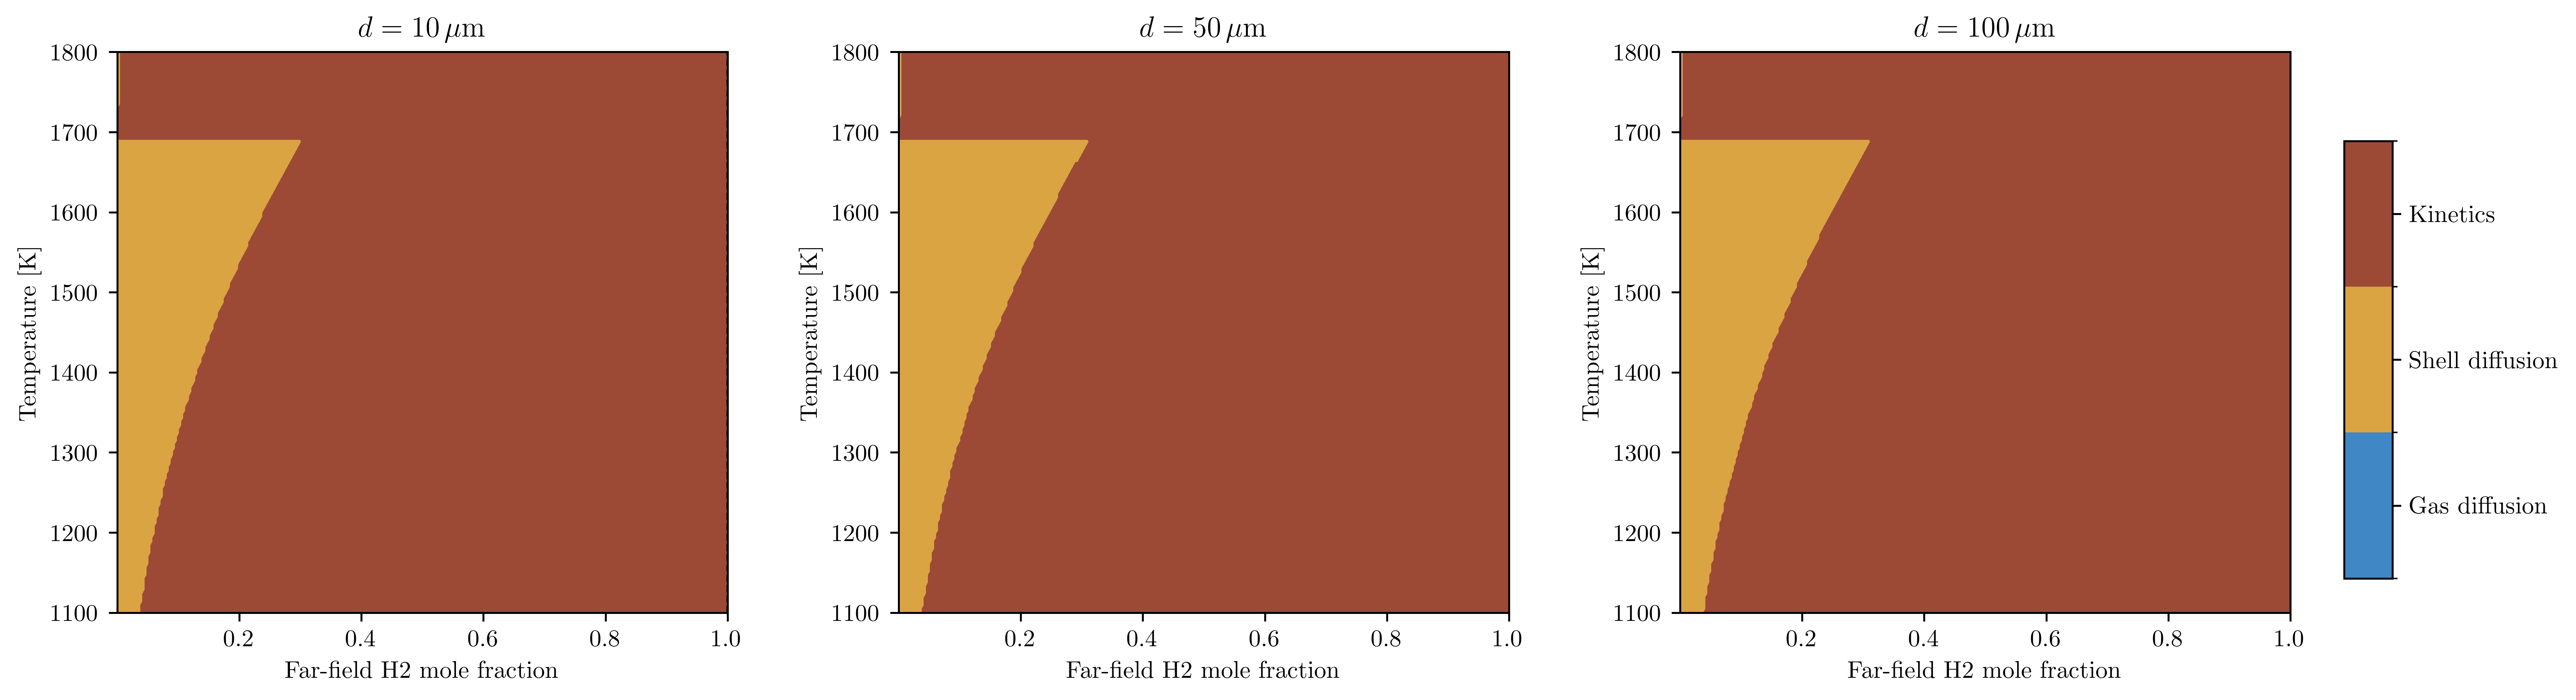
\includegraphics[width=\textwidth]{limitation_maps_by_size.png}
\caption{Dominant limiting mechanism as a function of temperature and far-field
hydrogen mole fraction for three particle diameters at \SI{1}{\atm}. The color
bar identifies whether the controlling resistance is gas diffusion, shell
diffusion, or interfacial kinetics.}
\label{fig:size-map}
\end{figure}

Figure~\ref{fig:pressure-map} addresses the question most directly relevant to
the use of hydrogen diluted in argon. When the total pressure is reduced, the
gas-diffusion contribution grows and the transport-controlled region expands.
When the total pressure is increased, the gas-side resistance becomes less
important and the map shifts toward kinetic control. Therefore hydrogen
dilution cannot be interpreted solely as a reduction in hydrogen availability.
Its effect depends on how dilution is introduced and on the accompanying total
pressure. A dilute mixture may still be mechanistically useful, but only if the
chosen operating point remains in the same regime as the higher-hydrogen case of
interest.

\begin{figure}[H]
\centering
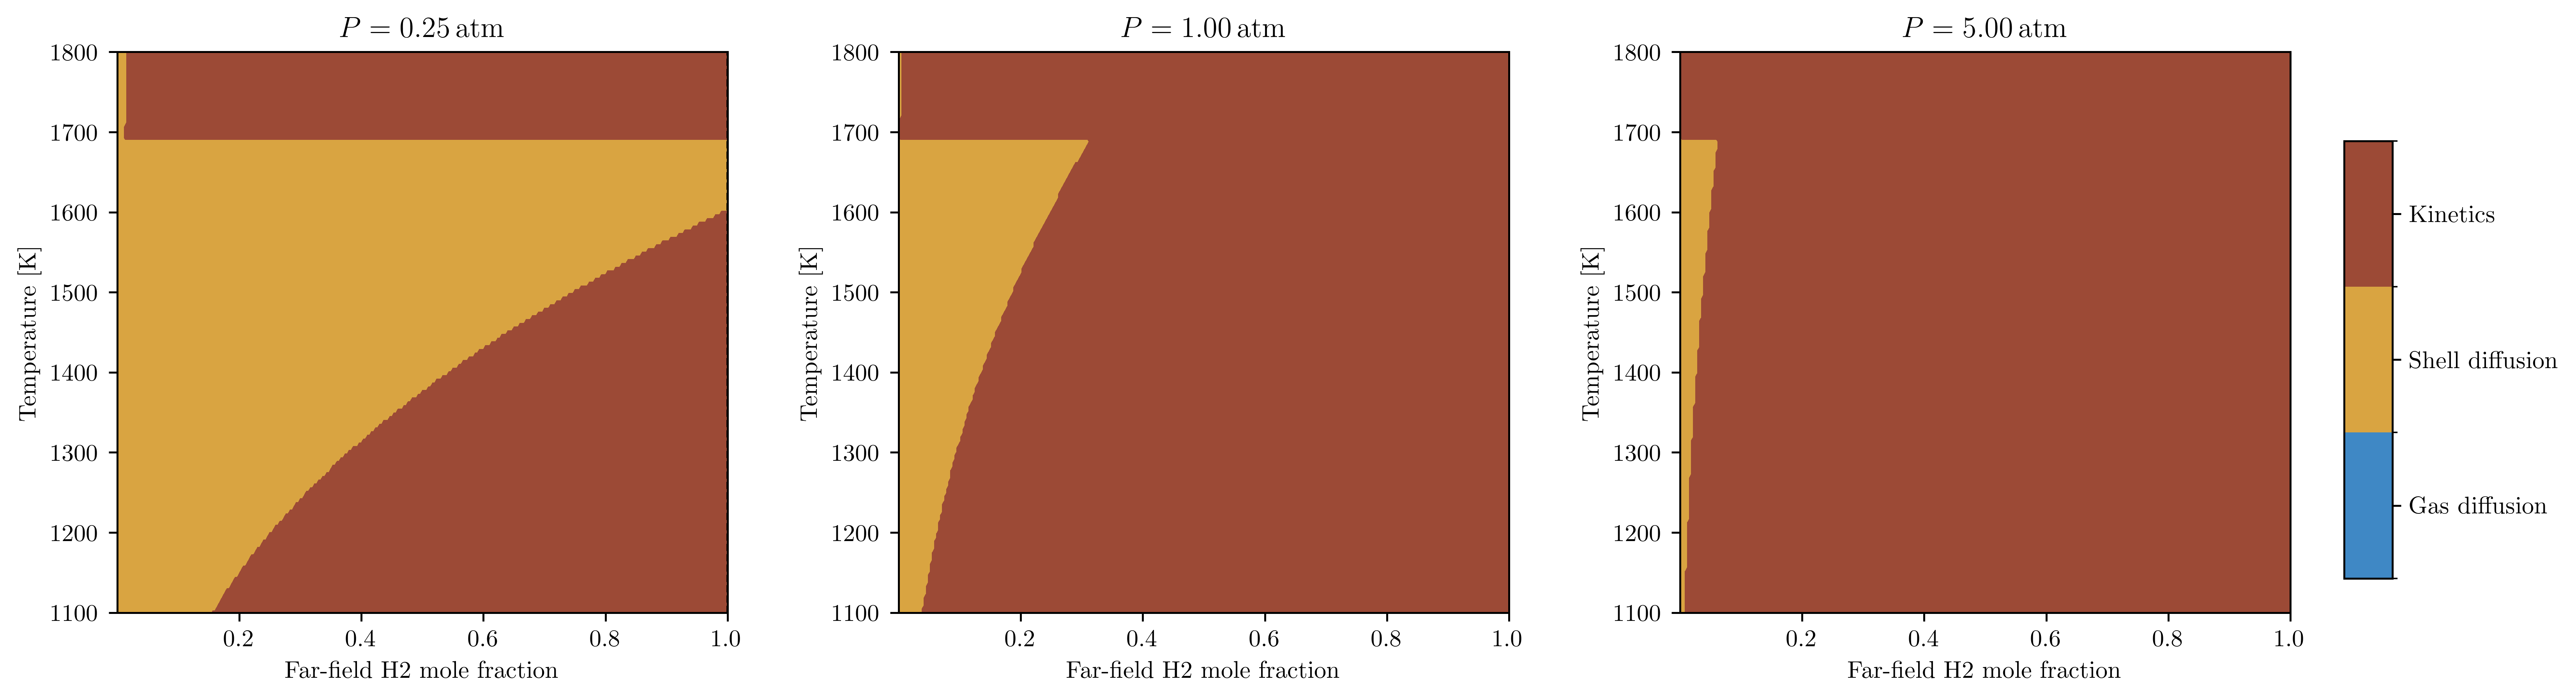
\includegraphics[width=\textwidth]{limitation_maps_by_pressure.png}
\caption{Effect of total pressure on the dominant limiting mechanism for a
\SI{50}{\micro\meter} particle. Lower total pressure broadens the region in
which transport, particularly shell diffusion and gas diffusion, is important,
whereas higher total pressure favors kinetic control in the present model.}
\label{fig:pressure-map}
\end{figure}

The quasi-steady radial profiles are shown in Fig.~\ref{fig:radial-profile} for
three far-field hydrogen mole fractions at \SI{1450}{\kelvin} and
\SI{1}{\atm}. The figure is divided into separate metal, shell, and gas
regions so that each spatial scale can be resolved clearly. Inside the metal,
the hydrogen level is taken to be zero in the present reduced description.
Inside the shell, the dashed curves represent the effective shell-side hydrogen
variable used in the diffusion model. Outside the particle, the solid curves
show the gas-phase hydrogen mole fraction. For the conditions shown here, the
gas-phase profile is nearly flat while the shell exhibits a much larger
gradient, reinforcing the conclusion that the shell resistance is often the
dominant transport contribution. Increasing the far-field hydrogen mole fraction
raises both the shell-side and gas-side levels, but it does not eliminate the
shell drop.

\begin{figure}[H]
\centering
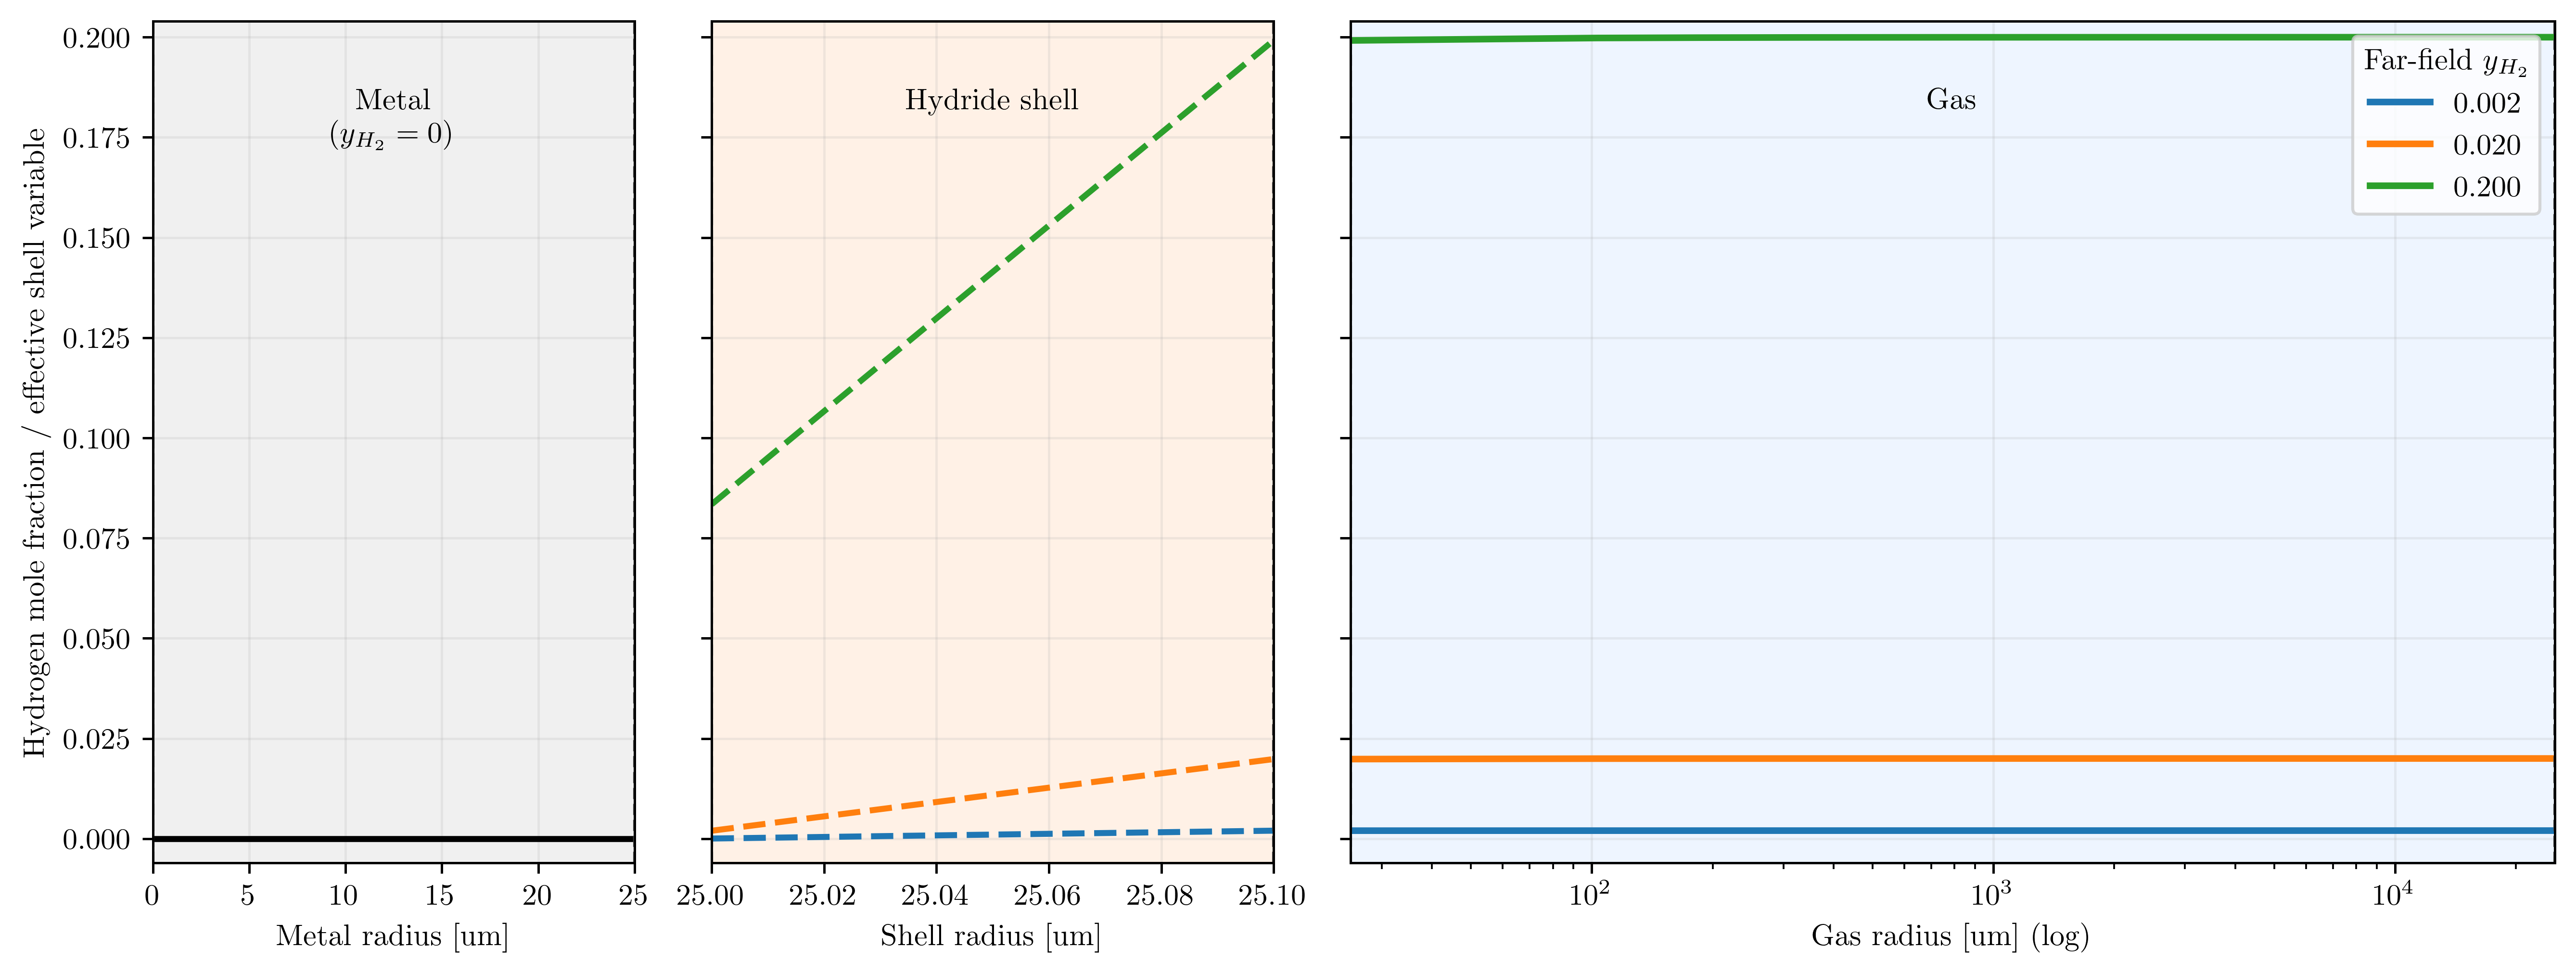
\includegraphics[width=\textwidth]{radial_profiles_by_yinf.png}
\caption{Quasi-steady hydrogen profiles in the metal, shell, and gas regions
for three far-field hydrogen mole fractions at \SI{1450}{\kelvin} and
\SI{1}{\atm}. Solid lines denote the gas-phase hydrogen mole fraction and
dashed lines denote the effective shell-side hydrogen variable for the same
condition.}
\label{fig:radial-profile}
\end{figure}

Taken together, these results support a practical interpretation for future
experimental design. If dilute \ce{H2}/Ar conditions are selected so that the
operating point remains within the same limiting region as the higher-hydrogen
condition of interest, then dilution may provide a safer route to performing still
mechanistically relevant experiments. If, however, dilution shifts the system
into a different controlling regime, then the resulting data may reflect a
different balance of physics and should not be treated as a simple surrogate for
the less diluted case.

\section{Limitations}

Several limitations should be emphasized. The model is quasi-steady and
isothermal, so it does not resolve thermal feedback from the reaction. The
hydride shell is represented by an effective diffusion law rather than a
detailed defect-transport model. The shell thickness is prescribed in the
baseline calculations rather than determined from a fully coupled moving-boundary
problem. Most importantly, the interfacial kinetics law is likely invalid since it is based
on solid-cerium data.\cite{Sarussi1993} The present results should therefore be
interpreted primarily as a mechanistic regime study rather than as a predictive
model of absolute hydriding rates. If a more accurate liquid hydriding kinetic mechanism can be found, replacing the existing model will be relatively trivial and the resulting predictions will be much more accurate.

\section{Conclusions}

The analysis presented here addresses whether hydrogen dilution in an
\ce{H2}/Ar mixture changes the limiting mechanism for cerium hydriding. Within
the quasi-steady framework used here, the answer is that dilution can change the
balance among gas diffusion, shell diffusion, and kinetics, especially when it
is accompanied by changes in total pressure. Shell diffusion is frequently the
dominant transport resistance for the baseline conditions examined, but kinetics
can become controlling at sufficiently high temperature and pressure, while
gas-phase diffusion becomes more relevant as total pressure decreases. The
practical implication is that dilute hydrogen experiments may still be useful
for future research, but only if the experimental conditions are chosen so
that the same limiting regime is preserved and the results are interpreted carefully.

\bibliographystyle{aiaa}
\bibliography{references}

\end{document}
